\documentclass[conference]{IEEEtran}
\IEEEoverridecommandlockouts
% The preceding line is only needed to identify funding in the first footnote. If that is unneeded, please comment it out.
\usepackage{cite}
\usepackage{amsmath,amssymb,amsfonts}
\usepackage{algorithmic}
\usepackage{graphicx}
\usepackage{textcomp}
\usepackage{xcolor}
\usepackage[spanish]{babel}
\usepackage{url}
\urlstyle{rm}

\usepackage{xspace}
\usepackage{color}

%Some comments
\newcommand\todo[1]{\mynote{TODO}{#1}}
\newcommand\wtf[1]{\mynote{WTF}{#1????}}
\newcommand\fix[1]{\mynote{FIX}{#1}}
\newcommand\reform[1]{\mynote{reform}{#1}} %reformulate
\newcommand{\here}[0]{\bigskip \mbox{\bf**************HERE*************}}

%Personal comments
\newcommand\pl[1]{\mynote{PL}{#1 }}
\newcommand\et[1]{\mynote{ET}{#1}}
\newcommand\hf[1]{\mynote{HF}{#1}}

%Connectors
\newcommand{\ie}[0]{{\em i.e.,~}}
\newcommand{\eg}[0]{{\em e.g.,~}}
\newcommand{\etal}[0]{{\em et al.}}
\newcommand{\aka}[0]{{\em a.k.a.}}
%\newcommand{\ala}[0]{{\em al a}}

%Languages
\newcommand{\javascript}[0]{\mbox{JavaScript}\xspace}
\newcommand{\deloreanjs}[0]{\mbox{DeloreanJS}\xspace}
\newcommand{\actionscript}[0]{\mbox{ActionScript}\xspace}
\newcommand{\java}[0]{\mbox{Java}\xspace}

%Aspect languages
\newcommand{\aspectscript}[0]{\mbox{AspectScript}\xspace}
\newcommand{\aspectj}[0]{\mbox{AspectJ}\xspace}


%Web
\newcommand{\async}[0]{\mbox{SyncAS}\xspace}
\newcommand{\promise}[0]{\mbox{Promise}\xspace}
\newcommand{\asyncjs}[0]{\mbox{Async.Js}\xspace}
\newcommand{\ajax}[0]{\mbox{Ajax}\xspace}
\newcommand{\synccc}[0]{\mbox{Sync/cc}\xspace}
\newcommand{\callcc}[0]{\mbox{continuations}\xspace}
\newcommand{\jquery}[0]{\mbox{jQuery}\xspace}
\newcommand{\rhino}[0]{\mbox{Rhino}\xspace}
\newcommand{\ecmascript}[0]{\mbox{ECMAScript}\xspace}
\newcommand{\browserify}[0]{\mbox{Browserify}\xspace}
\newcommand{\unwinder}[0]{\mbox{Unwinder}\xspace}
\newcommand{\nodejs}[0]{\mbox{Nodejs}\xspace}
\newcommand{\tongoy}[0]{\mbox{Tongoy-UCN}\xspace}


%==================================================
%Helper commands
\definecolor{red}{rgb}{1,0,0}
\newcommand\change[1]{\textcolor{red}{#1}}
\newcommand{\kw}[1]{{\bf#1}}
\newcommand{\parhead}[1]{\noindent{\bf {\em #1.}}}

\newcommand{\mynote}[2]{
\fbox{\bfseries\sffamily\scriptsize#1}
  {\small\textsf{\emph{#2}}}
\fbox{\bfseries\sffamily\scriptsize }
}

\newcommand{\super}[1]{\ensuremath{^{\textrm{#1}}}}
\newcommand{\sub}[1]{\ensuremath{_{\textrm{#1}}}}

\usepackage{graphicx}
\usepackage{xspace}
%\usepackage{url}
\usepackage{listings}
% The following packages are used in the Scheme definition


\lstdefinelanguage{java}{
morekeywords={%Java keywords
float, public, interface, class, static, void, extends, implements, final,
boolean, return, new, abstract, super, for, int, package, private, import,
protected, this, throw, try, finally, if, else, while, instance of, &&, ||},
	sensitive=true,
	morecomment=[l]{//},
	morecomment=[s]{/*}{*/},
	morestring=[b]",
}

\lstdefinelanguage{tracematches}
{morekeywords={%Java keywords
float, public, interface, class, static, void, extends, implements, final,
boolean, return, new, abstract, super, for, int, package, private, import,
protected, this, throw, try, finally, if, else, while, instance of, &&, ||,
%Aspectj keywords
before, around, after, returning, tracematch, sym, call, exec},
	sensitive=true,
	morecomment=[l]{//},
	morecomment=[s]{/*}{*/},
	morestring=[b]",
}


\lstdefinelanguage{JavaScript}
	{morekeywords={%Java keywords
	               true, false, return, new, function, var,
	               this, throw, try, finally, if, else, while, for, instanceof, 
	               %Others
	               async, await},
	sensitive=true,
	morecomment=[l]{//},
	morecomment=[s]{/*}{*/},
	morestring=[b]",
}

\lstset{
	frame=,
	language=JavaScript,
	xleftmargin=6pt,
	stepnumber=1,
	numbers=none,
	numbersep=5pt,
	numberstyle=\ttfamily\tiny,
	belowcaptionskip=\bigskipamount,
	captionpos=b,
	escapeinside={*'}{'*},
	tabsize=2,
	emphstyle={\bf},
	stringstyle=\mdseries\rmfamily,
	showspaces=false,
	keywordstyle=\bfseries,
    basewidth=0.5em,
	columns=fixed,
	%basicstyle=\footnotesize\sffamily,
         basicstyle=\scriptsize,
	showstringspaces=false,
	morecomment=[l]\%,
	commentstyle=\it
}

%\newcommand{\co}[1]{\mbox{{\small #1}\xspace}}
\newcommand{\co}[1]{\mbox{{\fontfamily{phv}\selectfont\scriptsize #1}\xspace}}
\newcommand{\env}[1]{\framebox{{\fontfamily{phv}\selectfont\scriptsize
#1}\xspace}}
\newcommand{\lambdac}[0]{$\lambda$~}
%\renewcommand{\ttdefault}{cmtt}
%\renewcommand{\ttdefault}{txtt}


\def\BibTeX{{\rm B\kern-.05em{\sc i\kern-.025em b}\kern-.08em
    T\kern-.1667em\lower.7ex\hbox{E}\kern-.125emX}}
\begin{document}

\title{DeloreanJS: Un Debugger en el Tiempo para JavaScript}

\author{\IEEEauthorblockN{Paul Leger}
\IEEEauthorblockA{\textit{Escuela de Ingenier\'ia} \\
\textit{Universidad Cat\'olica del Norte}\\
Coquimbo, Chile \\
pleger@ucn.cl}
\and
\IEEEauthorblockN{Felipe Ruiz}
\IEEEauthorblockA{\textit{Escuela de Ingenier\'ia} \\
\textit{Universidad Cat\'olica del Norte}\\
Coquimbo, Chile \\
felipe.ruiz@alumnos.ucn.cl}
\and
\IEEEauthorblockN{Guillermo Victorero}
\IEEEauthorblockA{\textit{Escuela de Ingenier\'ia} \\
\textit{Universidad Cat\'olica del Norte}\\
Coquimbo, Chile \\
guillermo.victorero@alumnos.ucn.cl}
}

\maketitle

\begin{abstract}
Aplicaciones Web, usando \javascript, son desarrolladas cada vez con mayor frecuencia. Como en la mayor\'ia de los entornos de desarrollos, una aplicaci\'on Web puede adquirir defectos de software (conocido como {\em bugs}), cuyos s\'intomas se aprecian durante el desarrollo e incluso, siendo peor, en producci\'on. Para ello, el uso de debuggers es sumamente \'util para detectar bugs. Lamentablemente, los actuales debuggers solamente avanzan hacia adelante en la ejecuci\'on para detectar un bug y no permiten retornar hacia un punto anterior en la ejecuci\'on para tomar acciones asociadas al bug detectado. Por ejemplo, probar si el mismo bug podr\'ia gatillarse con otro valor de una variable. Usando el concepto de continuaciones, este art\'iculo presenta un debugger para \javascript, llamado \deloreanjs, que permite a un programador volver en el tiempo en la ejecuci\'on con el fin pueda volver y probar el contexto alrededor de un bug. Este debugger ha sido implementado como una prueba de concepto en una extensi\'on para Google Chrome.         
\end{abstract}

\begin{IEEEkeywords}
\deloreanjs, \javascript, Debugger, Web application, Continuations
\end{IEEEkeywords}

\section{Introducci\'on}
\label{sec:intro}

Para construir aplicaciones Web, uno de los lenguajes m\'as usados es \javascript, cuya presencia en el entorno de la Web es de alrededor del 95\%~\cite{jsuses}. Asimismo, la industria del software se mueve fuertemente hacia el desarrollo de este tipo de aplicaciones, siendo testigo un gran n\'umero de migraciones de aplicaciones {\em standalone} a la Web; los ejemplos van desde convertir un documento Word a un formato PDF~\cite{smallpdf} hasta un sistema online ERP ({\em Enterprise Resource Planning})~\cite{erpOrcale}. Por ello, cada vez estas aplicaciones se han vuelto m\'as complejas y con mayor riesgo de introducir defectos de software (\aka {\em bugs}). 

Detectar y reparar bugs representa una de las tareas m\'as costosa en el proceso de desarrollo de software, y las aplicaciones Web no son la excepci\'on. Para aliviar el proceso de tratamiento de bugs, un conjunto de debuggers han sido propuestos, desde el que incluye un navegador en su distribuci\'on (\eg Mozilla Firefox developer tools) hasta  debuggers omniscientes que pueden recorrer a trav\'es de la traza de ejecuci\'on de una aplicaci\'on para encontrar las causas de un bug~\cite{azar:2016,barrAl:fse2016}. Considerando estos \'ultimos debuggers, ellos son {\em post-morter}, y es decir, solo permiten mostrar la ocurrencia de un bug sin entregar la posibilidad de retroceder {\em en el tiempo} las veces necesarias para que un programador pueda repararlo mientras la aplicaci\'on se ejecuta o manipular los valores de las variables alrededor del bug para mejorar la comprensi\'on de su causa.       

Este art\'iculo cient\'ifico presenta \deloreanjs, un debugger que permite al desarrollador de una aplicaci\'on Web escrita en \javascript expresar al insercci\'on de {\em timepoints} (en cambio de {\em breakpoints}) para entregar la posibilidad retornar en el tiempo a esos puntos y modificar valores de variables para continuar la ejecuci\'on del programa. Este novedoso enfoque de \deloreanjs permite tres caracter\'isticas:    

\begin{enumerate}
	
	\item Modificar reiteradamente los valores de las variables asociado a un bug encontrado para mejorar la comprensi\'on de \'este. Lo anterior puede ahorrar un gran n\'umero de ejecuciones usando un contexto similar para descubrir la verdadera raz\'on del bug.

	\smallskip

	\item Probar escenarios hipot\'eticos de la ejecuci\'on de una aplicaci\'on Web usando un timepoint de \deloreanjs. Esto permite explorar diversas evoluciones de la ejecuci\'on de la aplicaci\'on cambiando valores de algunas de sus variables.
   
   \smallskip
	 
	\item Mantener una aplicaci\'on Web funcionando usando los timepoints para potencialmente reparar un bug durante la ejecuci\'on. Lo anterior significa que no es siempre necesario detener la ejecuci\'on de la aplicaci\'on con el fin de realizar un anal\'isis post-morter.  

\end{enumerate}


Para construir \deloreanjs, utilizamos la abstracci\'on {\em continuaci\'on}~\cite{fw84} de los lenguajes de programaci\'on funcional como Scheme~\cite{scheme48}. Una continuaci\'on permite al programador capturar y guardar, como valor del lenguaje, un momento en la ejecuci\'on ({\em contador de programa} y {\em pila}) de una aplicaci\'on. Extendiendo esta abstracci\'on para lenguajes no funcionales como \javascript, nosotros habilitamos a \deloreanjs para que ofrezca la posibilidad a un programador de expresar la insercci\'on de timepoints en una aplicaci\'on Web,  y as\'i poder volver esos momentos de ejecuci\'on y modificarlos cuando es requerido.   


El art\'iculo est\'a organizado como sigue. La secci\'on~\ref{sec:tour} presenta diferentes ejemplos de aplicaci\'on de \deloreanjs, donde se puede apreciar la interfaz gr\'afica de nuestra propuesta. Luego, se presenta \deloreanjs, detallando c\'omo se usa y extiende continuaciones, y la integraci\'on con un navegador. En la secci\'on~\ref{sec:rw} se discuten debuggers similares. Finalmente, secci\'on~\ref{sec:conc} concluye y describe lineamientos sobre el trabajo futuro de nuestra propuesta.      

\smallskip

{\bf {\em Disponibilidad.}} El c\'odigo fuente de la implementaci\'on de \deloreanjs se encuentra en {\tt \url{http://github.com/fruizrob/delorean}}. Adem\'as, los ejemplos presentados aqu\'i se pueden probar online sin la necesidad de una ninguna extensi\'on en el sitio Web de nuestra propuesta {\tt \url{http://pleger.cl/delorean}}~\cite{deloreanjs}.

\section{Un Tour por \deloreanjs}
\label{sec:tour}

Nosotros presentamos \deloreanjs a trav\'es de tres ejemplos concretos. Cada ejemplo aborda una de las tres caracter\'isticas de nuestra propuesta y pueden ser probados online en~\cite{deloreanjs}.     



\subsection{Ejemplo 1}
\label{sec:tour1}

\pl{Explicar con imag\'enes el ejemplo 1}

\subsection{Ejemplo 2}
\label{sec:tour2}

\pl{Explicar con imag\'enes el ejemplo 2}

\subsection{Ejemplo 3}
\label{sec:tour3}

\pl{Explicar con imag\'enes el ejemplo 3}

\bigskip

\begin{figure*}[t]
\begin{center}
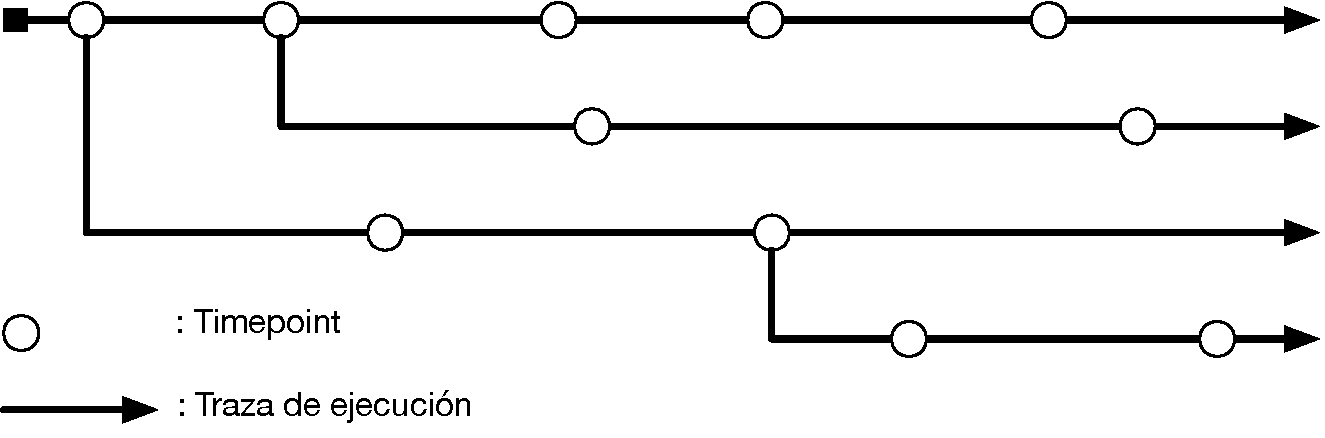
\includegraphics[width=.7\linewidth]{fig-timeline}
\caption{Multiples trazas de ejecuciones de la ejecuci\'on de una aplicaci\'on con \deloreanjs.}
\label{fig:timeline}
\end{center}
\end{figure*}


\begin{figure}[t]
\begin{center}
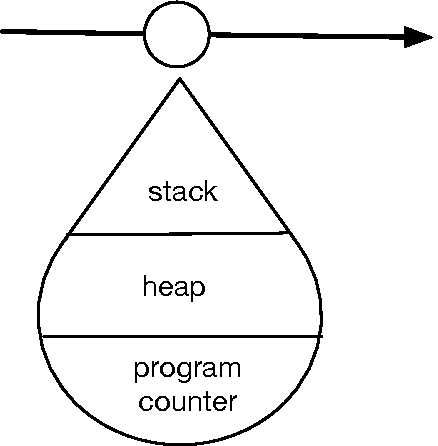
\includegraphics[width=.55\linewidth]{fig-timepoint}
\caption{Composici\'on de un timepoint, el cual es creado usando continuaciones y anal\'isis est\'atico del c\'odigo.}
\label{fig:timepoint}
\end{center}
\end{figure}


\section{\deloreanjs}
\label{sec:deloreanjs}

Dado que \deloreanjs propone un novedoso enfoque con respecto a los existentes debuggers, esta secci\'on describe c\'omo funciona. 

\smallskip

La figura~\ref{fig:timeline} muestra las multiples trazas de ejecuci\'on, llamadas {\em timelines}, que pueden ser producidas por los timepoints en una aplicaci\'on Web. Cuando un programador inserta un timepoint, se puede volver a ese timepoint durante la ejecuci\'on en el momento que una excepci\'on es gatillada, y as\'i crear una nueva timeline. Cada timeline representa una traza de ejecuci\'on distinta, por ejemplo, las variables \co{x} e \co{y} de la figura contienen distintos valores. A su vez, cada timeline puede generar otras timelines debido al uso de los timepoints insertados. 

\subsection{Construyendo Timepoints}
\label{sec:ctime}


%Como se puede apreciar en la figura~\ref{fig:timepoint}

Para permitir volver en el tiempo en una ejecuci\'on en \deloreanjs, la abstracci\'on de un timepoint es crucial (Figura~\ref{fig:timeline}). Esto es porque un timepoint captura y almacena el estado de la ejecuci\'on de una aplicaci\'on Web en t\'erminos del {\em program counter} (contador de programa), {\em stack} (pila), y {\em heap} (datos). En la figura~\ref{fig:timepoint} se puede apreciar que el program counter y stack es capturado usando continuaciones~\cite{fw84} y el heap es capturado a trav\'es de un an\'alisis est\'atico usando Babel~\cite{mckenzie:babel}.        
  
 \bigskip

\subsubsection{Capturando Program Counter y Stack}
\label{sec:continuaciones}

\begin{figure*}[t]
\begin{center}
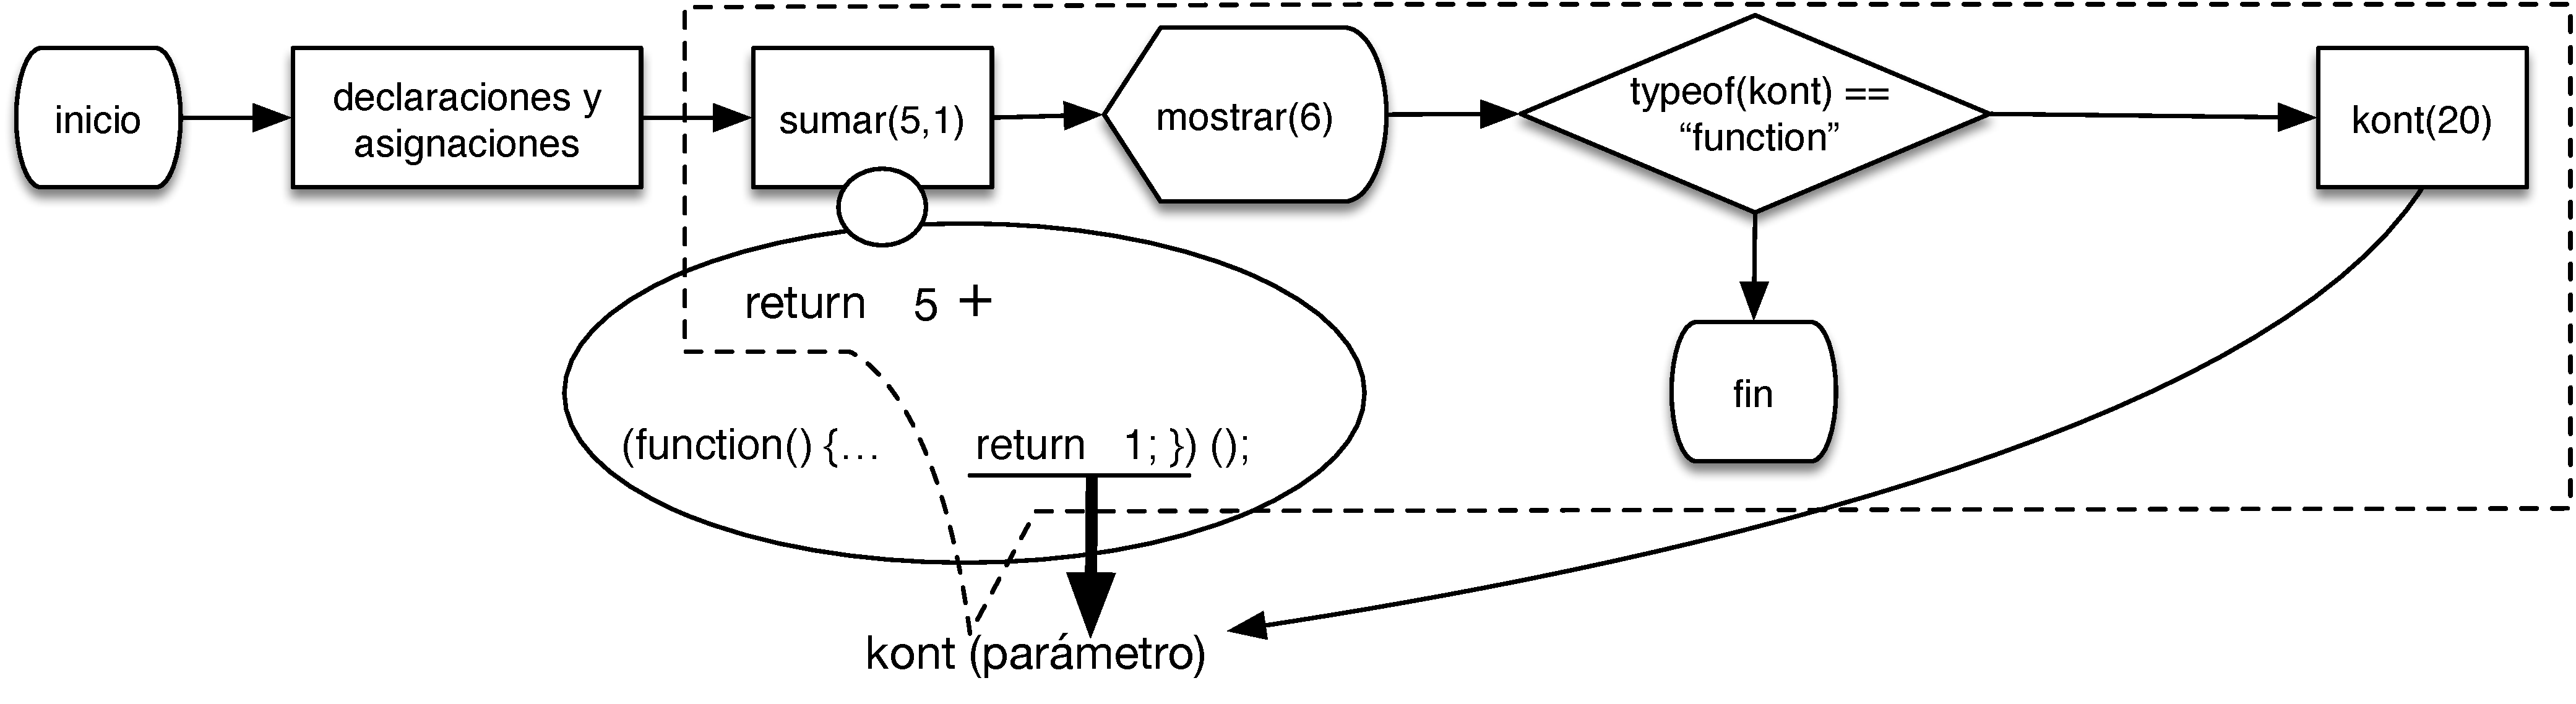
\includegraphics[width=.8\linewidth]{fig-kont}
\caption{El diagrama de flujo de la pieza c\'odigo ejemplifica continuaciones usando una continuaci\'on \co{kont}. La invocaci\'on de \co{kont} usa un \co{parametro} para reemplazar el retornado valor de la funci\'on an\'onima dentro de \co{sumar} (Figura elaborada desde~\cite{legerFukuda:sac-se2017}).}  

%\caption{The flowchart of Listing~\ref{lst:rhino_1}, which uses the continuation
 % \co{kont}. The invocation of \co{kont} uses a \co{parameter} to replace the
%  return value of the anonymous function inside of \co{add} (\ie ``\co{return 1}'').}
\label{fig:kont}
\end{center}
\end{figure*}

%Esta secci\'on brevemente introduce continuaciones y explica c\'omo son usadas por \deloreanjs. 

Para entender c\'omo estos dos elementos son capturados y almacenados, es necesario entender continuaciones. Los lenguajes de programaci\'on funcionales como Scheme~\cite{scheme48}, los cuales se caracterizan por no tener variables {\em mutables}, proveen una abstracci\'on llamada continuaci\'on. Esta abstraci\'on captura el program counter y stack de un programa funcional, y lo guarda como un {\em valor de primera clase}, es decir, un valor que soporta operaciones de asignaci\'on e invocaci\'on (ej. funciones en \javascript). Cuando una continuaci\'on es creada y guardada, \'esta puede ser invocada para reemplazar la actual ejecuci\'on del programa por la que est\'a guardada en la continuaci\'on. \unwinder~\cite{unwinder:2018} es una librer\'ia en \javascript que soporta continuaciones a trav\'es de una funci\'on llamada \co{callCC}. Nosotros ejemplificamos continuaciones con \unwinder usando una pieza de c\'odigo que captura la ejecuci\'on de una funci\'on que suma dos n\'umeros:     

%\break

%\begin{lstlisting}[linewidth=\columnwidth,numbers=left,caption=Uso de continuaciones con la librer\'ia \unwinder., label=lst:rhino_1]

\begin{lstlisting}[linewidth=\columnwidth,numbers=left]
var kont;

function sumar(x,y) {
  return x + (function() {
                kont = callCC(cont => cont);
                return typeof(kont) == "number"? kont:y;})();
}

mostrar(sumar(5,1));                           //muestra 6
if (typeof(kont) == "function") kont(20);      //muestra 25
\end{lstlisting}

La figura~\ref{fig:kont} muestra el diagrama de flujo de la pieza de c\'odigo anterior. En la l\'inea~5, una continuaci\'on \co{kont} es creada antes de sumar la variable \co{y}. Esta captura toma lugar en la l\'inea~9 cuando la funci\'on \co{sumar} es llamada. El resultado de \co{sumar} es pasado a \co{mostrar}, y se muestra el n\'umero \co{6}. La l\'inea~10 invoca la continuaci\'on asociada a \co{kont} con el par\'ametro \co{20}, produciendo que el valor retornado de la funci\'on an\'onima de las lineas~4-6 sea \co{20} y no \co{1}. Como resultado, se muestra \co{25} (\co{25 = (x = 5) + (y = 20)}). Notar que el {\em if expression}~(l\'inea~6) y {\em if statement}~(l\'inea~10) son usadas para diferenciar entre la creaci\'on de una continuaci\'on y su invocaci\'on. Una continuaci\'on es una funci\'on (l\'inea~9) cuando es creada, y cuando es invocada es enlazada al valor pasado como par\'ametro (ej. el valor \co{20} en esta pieza de c\'odigo).         

%\here

%Figure~\ref{fig:kont} shows a flowchart of the piece of code above. In Line~5,
%the piece of code captures and stores the continuation in \co{kont} before
%adding \co{y}. This capture takes place in Line~9 when \co{add} is called.  The
%result of \co{add} is passed to \co{show}, and then the number \co{6} is
%displayed.  Line~10 executes the continuation bound to \co{kont} with \co{20} as
%parameter, which replaces the return of the anonymous function of Line~6 (\ie
%\co{return 1} $\rightarrow$ \co{return 20}). As a result, \co{25} is displayed
%(\co{25 = (x = 5) + (y = 20)}). Note that the {\em if expression} (Line~6) and
%{\em if statement} (Line~10) are used to differentiate when a continuation is
%created from being called. A continuation is a function (Line~9) if this
%continuation has been created but not called, otherwise the continuation is
%bound to the value passed by parameter when it is called (\ie~20 in this piece
%of code).

%If developers need to stop a handler execution, a continuation in the end of the
%top-level script should be created. For example, Listing~\ref{lst:rhino_2}:
%
%\begin{lstlisting}[caption=Stopping a \javascript script with continuations., label=lst:rhino_2]
%function showMessageHandler() {
%  show("This message will be shown");
%  stop();
%  show("This message will never be shown");
%}
%
%var stop = callCC(cont => cont);
%\end{lstlisting}
%
%\synccc uses two continuations: the first one stops a handler execution just
%after an asynchronous operation invocation, and the second one resumes the
%handler execution when the asynchronous operation response is available.

\bigskip

\subsubsection{Capturando el Heap}
\label{sec:heap}

\begin{figure}[t]
\begin{center}
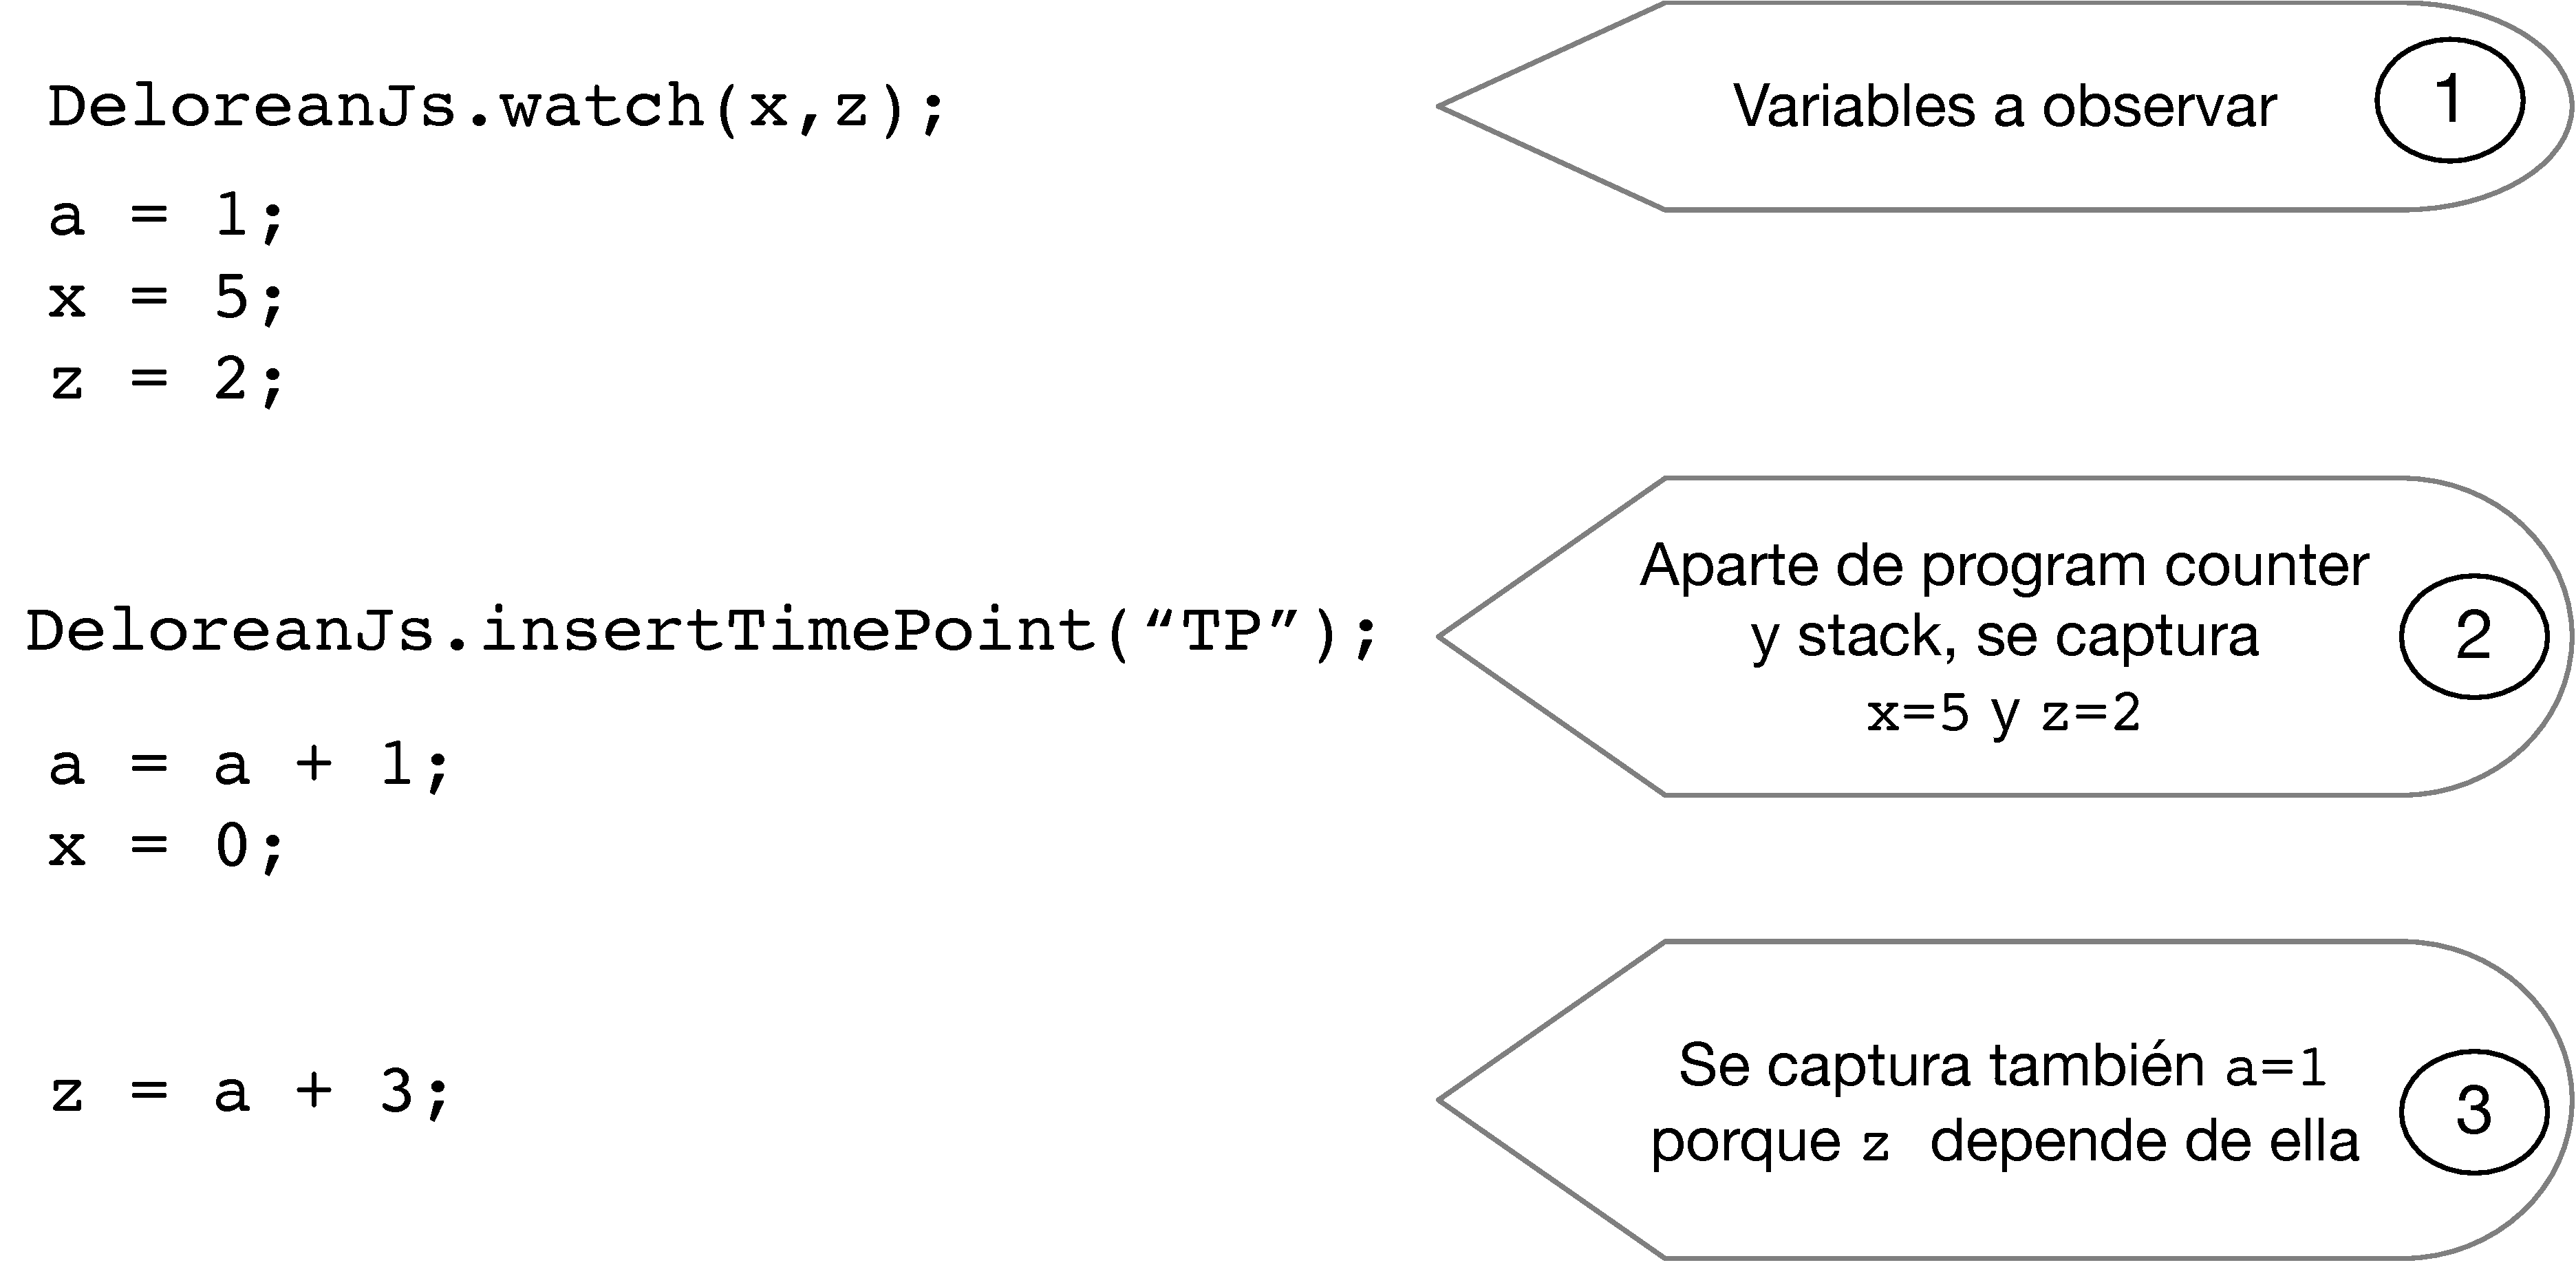
\includegraphics[width=.8\linewidth]{fig-heap1}
\caption{Las tres etapas para capturar y almacenar las variables observadas (ej. \co{x} y \co{z}) y las variables que pueden modificar a ellas (ej. la variable \co{a} porque modifica \co{z}).}
\label{fig:heap1}
\end{center}
\end{figure}


\begin{figure}[t]
\begin{center}
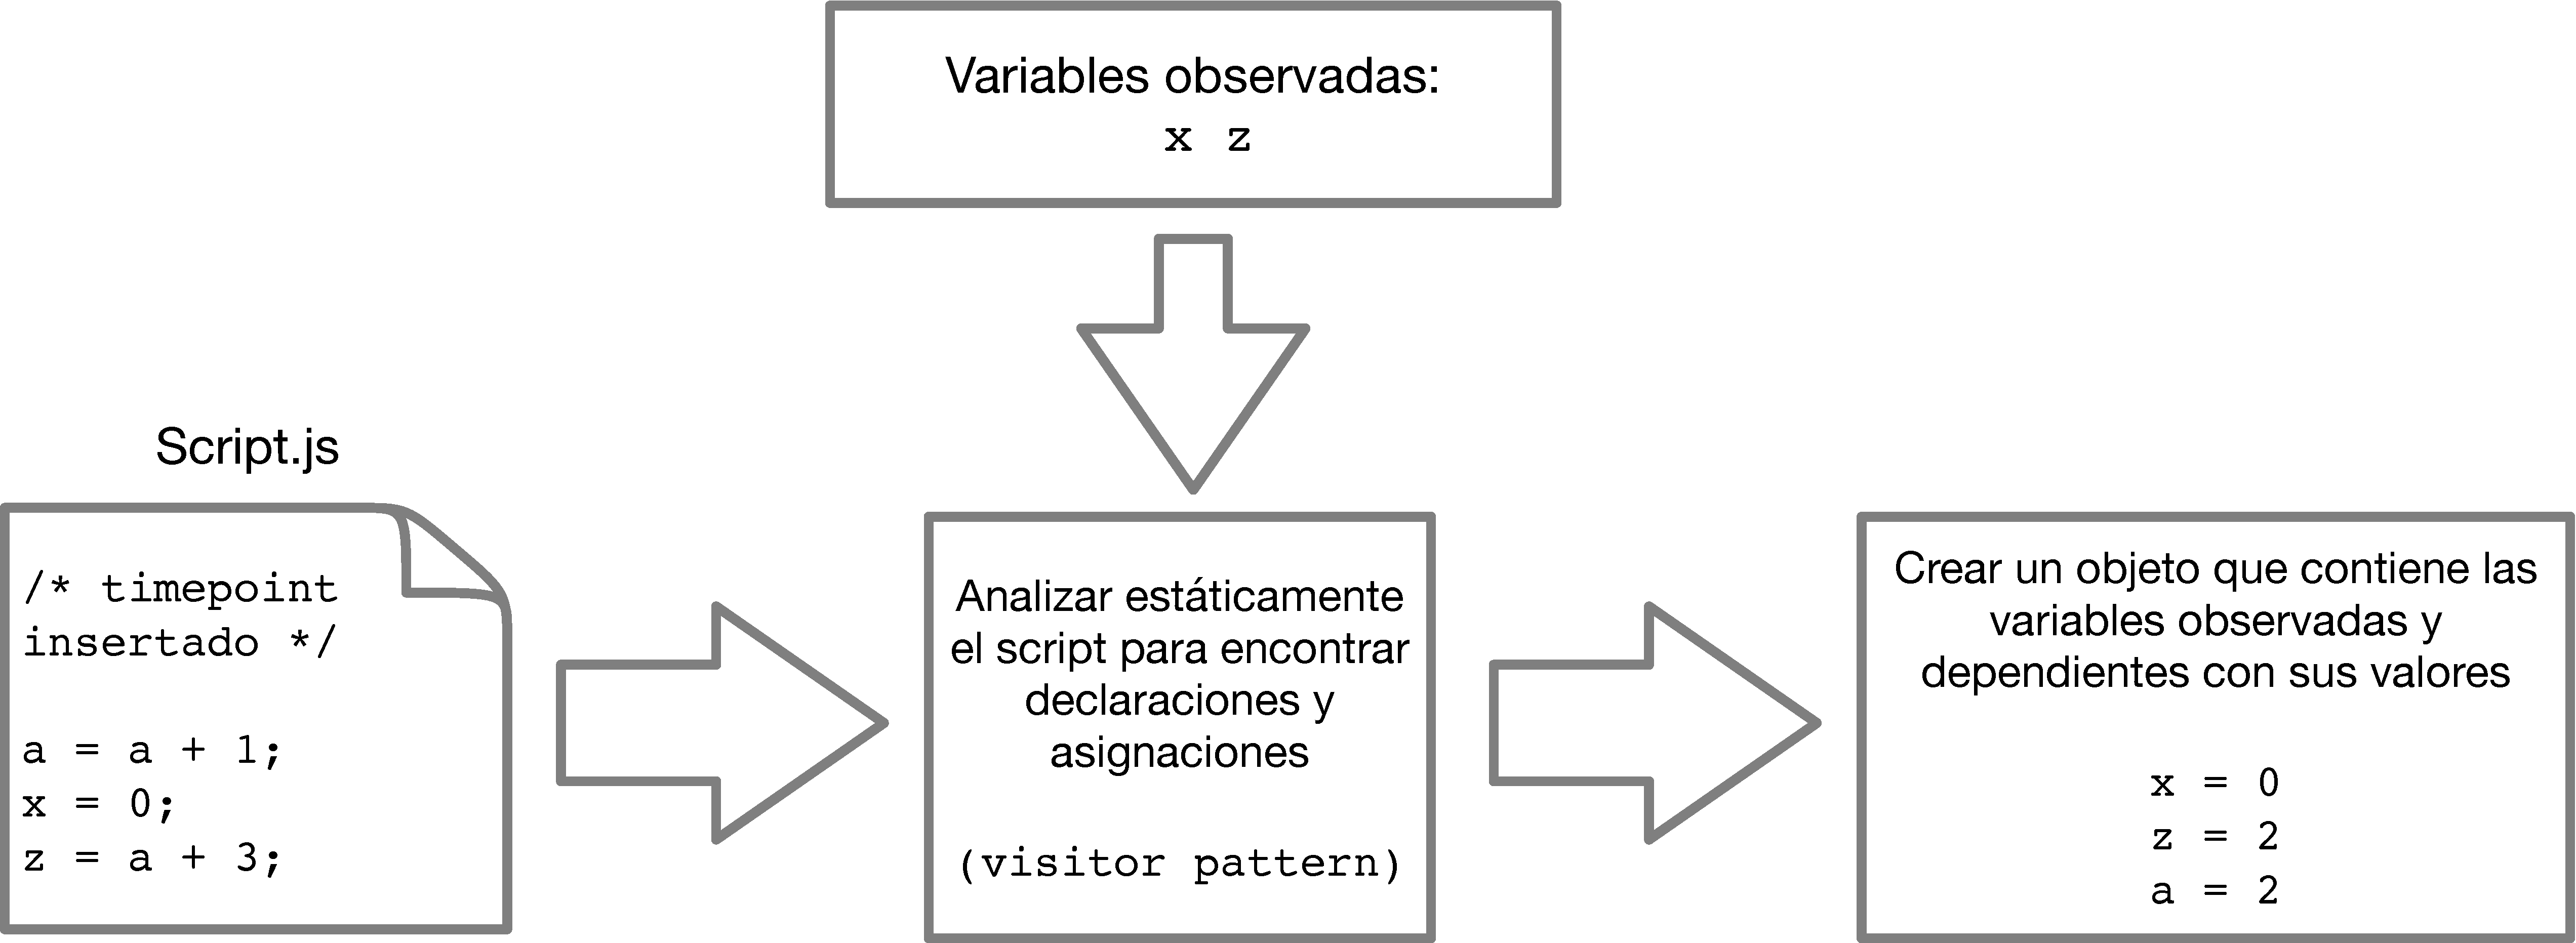
\includegraphics[width=.8\linewidth]{fig-heap2}
\caption{.}
\label{fig:heap2}
\end{center}
\end{figure}

Un timepoint tambi\'en necesita capturar y almacenar las variables que se encuentran en el heap, pero lamentablemente una continuaci\'on no lo realiza. Para lograrlo, antes de ejecutar una aplicaci\'on Web, \deloreanjs realiza un an\'alisis est\'atico para capturar las variables del heap con sus valores que han sido {\em observadas} por el programador que usa nuestra propuesta. La figura~\ref{fig:heap1} ejemplifica las tres etapas que debe realizar el an\'alisis est\'atico para capturar las variables. En la etapa 1, se definen las variables del heap que deben ser observadas (\co{x} y \co{z}). Luego en la etapa 2, se captura y almacena los valores de las variables previamente definidas. Finalmente en la etapa 3, se puede apreciar que las variables que modifican a las variables observadas tambi\'en son capturadas y almacenadas (\co{a}). Esta \'ultima etapa es necesaria porque se debe asegurar que las variables observadas deben potencialmente comportarse igual (es decir, con los mismos valores) cuando una ejecuci\'on comienza desde un timepoint; en el ejemplo de la figura, si \co{a} no es capturado, entonces \co{z} tendr\'ia un distinto valor cuando una ejecuci\'on vuelva a comenzar desde el timepoint.          

Para lograr las etapas de la figura~\ref{fig:heap1}, \deloreanjs usa el {\em Visitor pattern}~\cite{GoF94} para realizar el an\'alisis est\'atico como se muestra en la figura~\ref{fig:heap2} usando la librer\'ia Babel~\cite{mckenzie:babel}. Con esta librer\'ia, nuestra propuesta examina cada sentencia del c\'odigo fuente de la aplicaci\'on para permite al programador acc    


\here

%Cada visitor busca expresiones de asignación y de declaración, respectivamente, a alguna de las variables a observar definidas por el usuario. Al encontrar una, añade todas las variables al lado derecho de la expresión al objeto dependencias.
%Cuando la ejecución llega a un timepoint, delorean obtiene los valores de cada variable a observar y de cada dependencia en ese instante y los guarda junto al nombre de la variable correspondiente. Cada timepoint genera y almacena un objeto con estos valores en ese momento.

%\pl{Explicar su forma de capturar estados}

\subsection{Usando Timepoints}
\label{sec:utime}

\pl{Explicar la aplicaci\'on cuando se interactua con el desarrollador}

\bigskip

\section{Trabajos Relacionados}
\label{sec:rw}

Debido a que \javascript es un lenguaje muy ampliamente usado, existe un inter\'es constante en crear avances en t\'erminos de investigaci\'on~\cite{vazquesAl:ist2018,legerAl:scp2013,legerAl:scp2015,zhengAl:www2011,chargueraudAl:www2018} y desarrollo~\cite{resig:jquery,angular,mckenzie:babel,rxjs}. En estos avances, varios tipos de propuestas de debuggers son posible encontrar en la literatura. Algunos de ellos~\cite{bartonOdvarko:www2011,jsbin,nodejsInspector} ofrecen un amplio conjunto de caracter\'isticas como modificar los valores de variables mientras la aplicaci\'on se est\'a ejecutando (ej. FireBug~\cite{bartonOdvarko:www2011}). Aunque, en lo mejor de nuestro conocimiento, no es encontrar debuggers que sigan un enfoque similar a \deloreanjs, existen algunos que consideran la historia de ejecuci\'on de una aplicaci\'on Web:       

\smallskip

\parhead{Debuggers omniscientes} Estos tipos de debuggers se encargan de almacenar cada evento que ocurre en la ejecuci\'on de un programa, creando un historial de la traza de ejecuci\'on. Estos debuggers han sido implementados en lenguajes como en \java~\cite{tod:oopsla2007} y xDSMLs~\cite{bousseAl:SLE2015}. Con respecto a  \javascript, podemos encontrar PECCit~\cite{azar:2016} y JARDIS~\cite{barrAl:fse2016}, los cuales almacenan la traza de ejecuci\'on y ofrecen diferentes interfaces de usuario para navegar a trav\'es de esta traza. A diferencia de \deloreanjs, estos tipos de debuggers son {\em post-morter}, significando que no es posible volver a un punto en la historia de esta ejecuci\'on y continuarla con valores de variables potencialmente modificados. 

\smallskip

\parhead{Debuggers remotos} \javascript es generalmente\footnote{Aparte de la Web, \javascript actualmente es usado en varios entornos de desarrollos, por ejemplo, es usado en el lado del servidor en una aplicaci\'on Web~\cite{nodejs:2018} y en administradores de ventas de sistemas operativos basados en Linux~\cite{gjs}.} usado para construir aplicaciones Web\ que son usadas por usuarios con alg\'un dispositivo que pertenece a un muy variado y amplio catalogo, pues lo \'unico que se necesita es un navegador con acceso a internet. Por esta raz\'on, cualquier configuraci\'on del dispositivo puede producir un potencial bug que los desarrolladores no podr\'ian observar en un ambiente de desarrollo controlado. Para abordar esta dificultad, existen debuggers~\cite{sessionstack,raygun,trackjs} que supervisan remotamente las ejecuciones de los usuarios. Similarmente a los debuggers omniscientes, estos registran y env\'ian cada punto ejecuci\'on a un desarrollador por la red. Aunque estos debuggers permiten a los desarrolladores trazas de ejecuciones de diferentes usuarios en tiempo real, no ofrecen la posibilidad de retroceder en momentos de la ejecuci\'on a los usuarios.   

\section{Conclusiones}
\label{sec:conc}


No es un misterio que la industria del software se est\'e orientando a construir aplicaciones Web cada vez m\'as grandes y complejas, implicando que exista una mayor probabilidad que aparezcan bugs. Para construir estas aplicaciones, el lenguaje \javascript es ampliamente usado y una amplia cantidad de debuggers se encuentra disponible en la Web~\cite{bartonOdvarko:www2011,jsbin,nodejsInspector,sessionstack,raygun,trackjs,azar:2016,barrAl:fse2016}. Sin embargo, a diferencia de \deloreanjs, ninguno de estos debuggers considera el enfoque de {\em retroceder en el tiempo} a momento en la ejeucuci\'on una aplicaci\'on escrita en \javascript. Sin este enfoque, hay un conjunto de oportunidades que un programador pierde, por ejemplo, probar distintos valores de variables en un mismo contexto de ejecuci\'on con el objetivo de mejorar la comprensi\'on del bug o explorar escenarios hipot\'eticos de la evoluci\'on de la ejecuci\'on dado un mismo contexto inicial. Para alcanzar una adopci\'on por parte de la comunidad, \deloreanjs tiene a\'un algunos desaf\'ios:  
   
\smallskip

\parhead{Capturar completamente el heap} A diferencia del stack que se captura autom\'aticamente en una aplicaci\'on en ejecuci\'on, un programador debe ahora especificar qu\'e variables del heap se guardar\'an en los timepoints. Resolver este desaf\'io implica almacenar copias de las variables contenidas en el heap por cada timepoint.      

\smallskip

\parhead{Integrar a un existente debugger} Actualmente \deloreanjs ofrece el nuevo enfoque de retroceder en el tiempo de una ejecuci\'on. Integrar este enfoque con las caracter\'isticas de los existentes debuggers podr\'ia significativamente la adopci\'on de nuestra propuesta. Por ejemplo, debuggers omniscientes integrado con \deloreanjs permitir\'ia analizar multiple trazas de ejecuciones partiendo desde un timepoint.

\smallskip

Como limitaci\'on podemos mencionar que \deloreanjs realiza la promesa de retornar en el tiempo de una ejecuci\'on, la cual podr\'ia no cumplirse a totalidad si aplicaci\'on depende de los resultados de eventos externos (ej. servicio Web que entrega la hora actual). Sin embargo, esta limitaci\'on se encuentra tambi\'en presenta en los existentes debuggers.               

\bibliographystyle{IEEEtran}
\bibliography{djs}


\end{document}
